\documentclass{article}
\usepackage{neurips_data_2024}
\usepackage[utf8]{inputenc} % allow utf-8 input
\usepackage[T1]{fontenc}    % use 8-bit T1 fonts
\usepackage{hyperref}       % hyperlinks
\usepackage{url}            % simple URL typesetting
\usepackage{booktabs}       % professional-quality tables
\usepackage{amsfonts}       % blackboard math symbols
\usepackage{nicefrac}       % compact symbols for 1/2, etc.
\usepackage{microtype}      % microtypography
\usepackage{xcolor}         % colors
\usepackage{lipsum}
\usepackage{graphicx}       % include pdfs as figures
\usepackage[ruled]{algorithm2e}
\usepackage{bm}

\title{\texttt{metabench}\\A Sparse Benchmark to Measure General Ability\\in Large Language Models}
\author{%
   Alex Kipnis $^{1}$ \thanks{Correspondence to \texttt{adkipnis@mailbox.org}} \quad
   Luca M. Schulze Buschoff $^{1}$ \quad
   Konstantinos Voudouris $^{1,2}$ \quad
   Eric Schulz $^1$\\
   $^1$ Human-Centered AI, Helmholtz Munich \quad $^2$ University of Cambridge\\
}

\begin{document}

\maketitle

\begin{abstract}
   Large Language Models (LLMs) vary in their abilities on a range of tasks. Initiatives such as the \texttt{Open LLM Leaderboard} aim to quantify these differences with several large benchmarks (sets of test items to which an LLM can respond either correctly or incorrectly).
   However, high correlations within and between benchmark scores suggest that (1) there exists a small set of common underlying abilities that these benchmarks measure, and (2) the latter tap into redundant information and may thus be considerably compressed.
   We use data from over $5.000$ LLMs to analyze the psychometric properties of six benchmarks (\texttt{ARC}, \texttt{GSM8K}, \texttt{HellaSwag}, \texttt{MMLU}, \texttt{TruthfulQA} and \texttt{WinoGrande}) in order to identify their most informative items.
   Using this subset, we construct a sparse benchmark, \texttt{metabench}, that has less than $4$\% of the original size of all six benchmarks combined. Moreover, \texttt{metabench} goes beyond point scores by yielding estimators of the underlying benchmark-specific abilities.
   We show that these estimators (1) can be used to reconstruct the original \textit{individual} benchmark scores, and (2) have one underlying common factor which can be used to reconstruct the original \textit{total} score with $\sim 2$\% error.
\end{abstract}

% ------------------------------------------------------------------------------------
% Introduction
\section{Benchmarks do not need to be big}
\lipsum[1]
\subsection{Related Work}
\lipsum[2]
% ------------------------------------------------------------------------------------
% Methods
\section{Benchmark Distillation}
\begin{figure}[h]
   \centering
   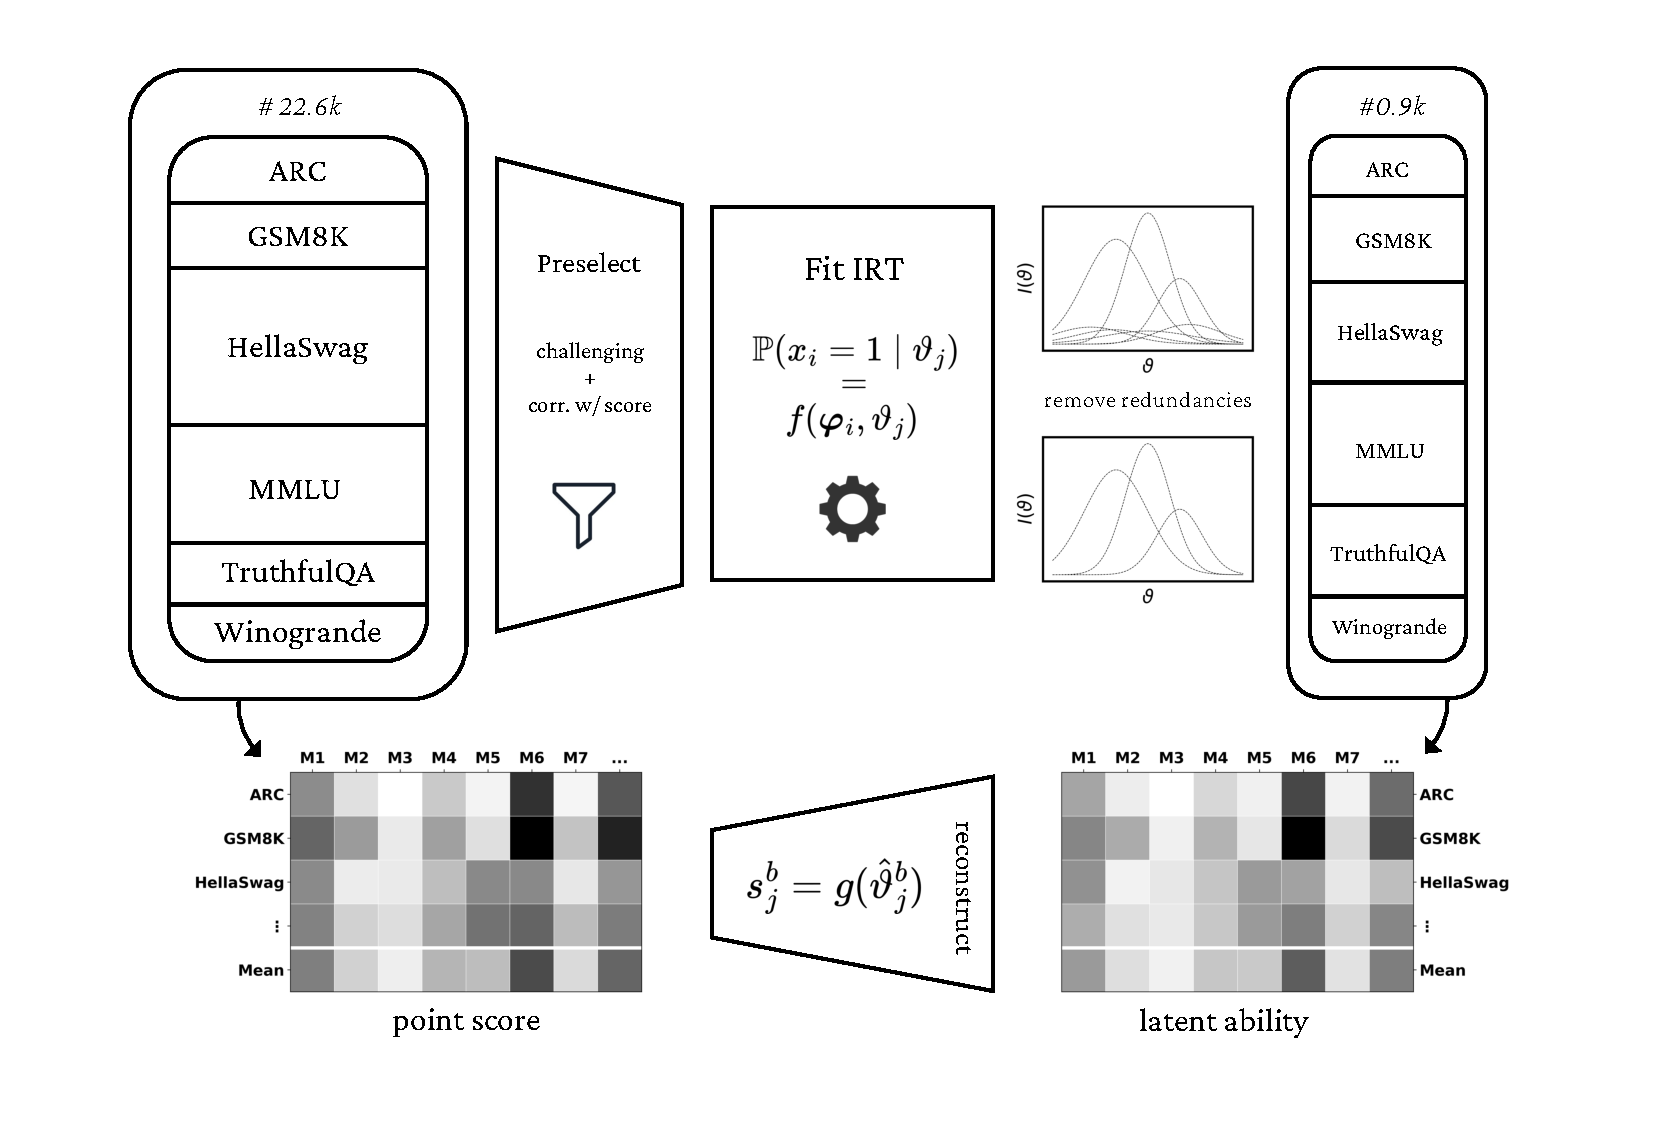
\includegraphics[width=0.8\textwidth]{figures/overview.pdf}
   \caption{\textit{Processing pipeline}. (1) Collect item-wise accuracies from all available LLMs for each benchmark on \texttt{Open LLM Leaderboard}. (2) Remove items solved by more than $95\%$ of LLMs and items with part-whole correlation $r \approx 0$. (3) Fit variants of IRT models to the remaining items and choose the best fit by cross-validation. (4) Infer item information from the item parameters and filter out uninformative items to (5) construct \texttt{metabench}. (6) Use the item parameters to estimate the benchmark-specific abilities and use factor analysis to find a common factor. (7) These can be used to reconstruct the original (normalized) benchmark scores as well as their mean.}
   \label{fig:overview}
\end{figure}
\subsection{Data Collection and Preprocessing}
% openllm leaderboard
We collected openly available item-wise accuracies from \href{https://huggingface.co/datasets}{Hugging Face Datasets} for the six benchmarks that are part of the \href{https://huggingface.co/open-llm-leaderboard}{\texttt{Open LLM Leaderboard}}: \texttt{ARC}, \texttt{GSM8K}, \texttt{HellaSwag}, \texttt{MMLU}, \texttt{TruthfulQA} and \texttt{WinoGrande}. % TODO: add citation
After excluding flagged and merged models, we obtained data from in total $6875$ LLMs, out of which $5055$ had data for all six benchmarks. For comparability, we normalized the benchmark scores on a percent scale and saved for future reference. Per benchmark, we removed LLMs with the lowest $0.1\%$ of scores to reduce noise.
Items with duplicate prompts, standard deviation below $1\%$ and easiness above $95\%$ were removed. We then estimated the part-whole correlation between  items and the total score using the point-biserial correlation coefficient:
\begin{equation}
   r_{pbis} = \frac{\mu_1 - \mu}{s_{n-1}} * \sqrt{\frac{n_1 * (n-n_1)}{n*(n-1)}},
\end{equation}
where $\mu_1$ resp. $\mu$ are the mean scores of the group who answered the item correctly resp. the total group, $s_{n-1}$ is the standard deviation of the total group, $n_1$ resp. $n$ are the size of the group that answered the item correctly resp. the total group. Items with $r_{pbis} = 0 \pm \epsilon$ were removed, $\epsilon$ was set to $0.05$ except for \texttt{Winogrande} where it was set to $0.02$ as otherwise hundreds of items would have been removed.\footnote{Note that it is customary to remove items with negative $r_{pbis}$. However, items with a negative $r_{pbis}$ \textit{do} contain information about the benchmark score. We therefore chose to keep them.}
For comparability, we conducted a train-test-validation split of the LLMs in the following manner: For stratification, we calculated the grand average (GA) of the original benchmark scores for models that had data for \textit{all six} benchmarks, and used it to split off $10\%$ of the LLMs for validation.For cross-validation per benchmark, we split off further $10\%$ of the remaining LLMs for testing, this time stratifying by the specific benchmark score. 

\subsection{Evolutionary Subsampling}
After preprocessing, \texttt{HellaSwag} and \texttt{MMLU} still had substantially more items than LLMs, prohibiting the use of IRT models. To further reduce their number of items to $1/4$ of the respectively available LLMs, we used an evolutionary subsampling approach:
\begin{enumerate}
   \item Randomly drop $k$ items from the benchmark.
   \item Re-calculate the mean score $\dot {\boldsymbol{\mu}}$ of the remaining items for each LLM.
   \item Fit a non-linear regression model on the training set: $\boldsymbol\mu = f(\dot{\boldsymbol\mu})$ 
   \item Calculate the root mean square error (RMSE) on the test subset.
\end{enumerate}
This inner loop is repeated $50$ times, and the iteration with the lowest RMSE makes the cut. The outer loop is repeated until the number of items reaches the goal size. The final set of items is also tested on the validation set. For \texttt{MMLU}, the procedure uses a linear model of all scenario scores to predict the total score, but is otherwise identical.
Using this procedure, we reduced the number of items in \texttt{HellaSwag} from $10042$ to $1181$ and in \texttt{MMLU} from $14042$ to $1108$ with minimal loss in predictive performance on the validation set.
\begin{figure}[h]
   \centering
   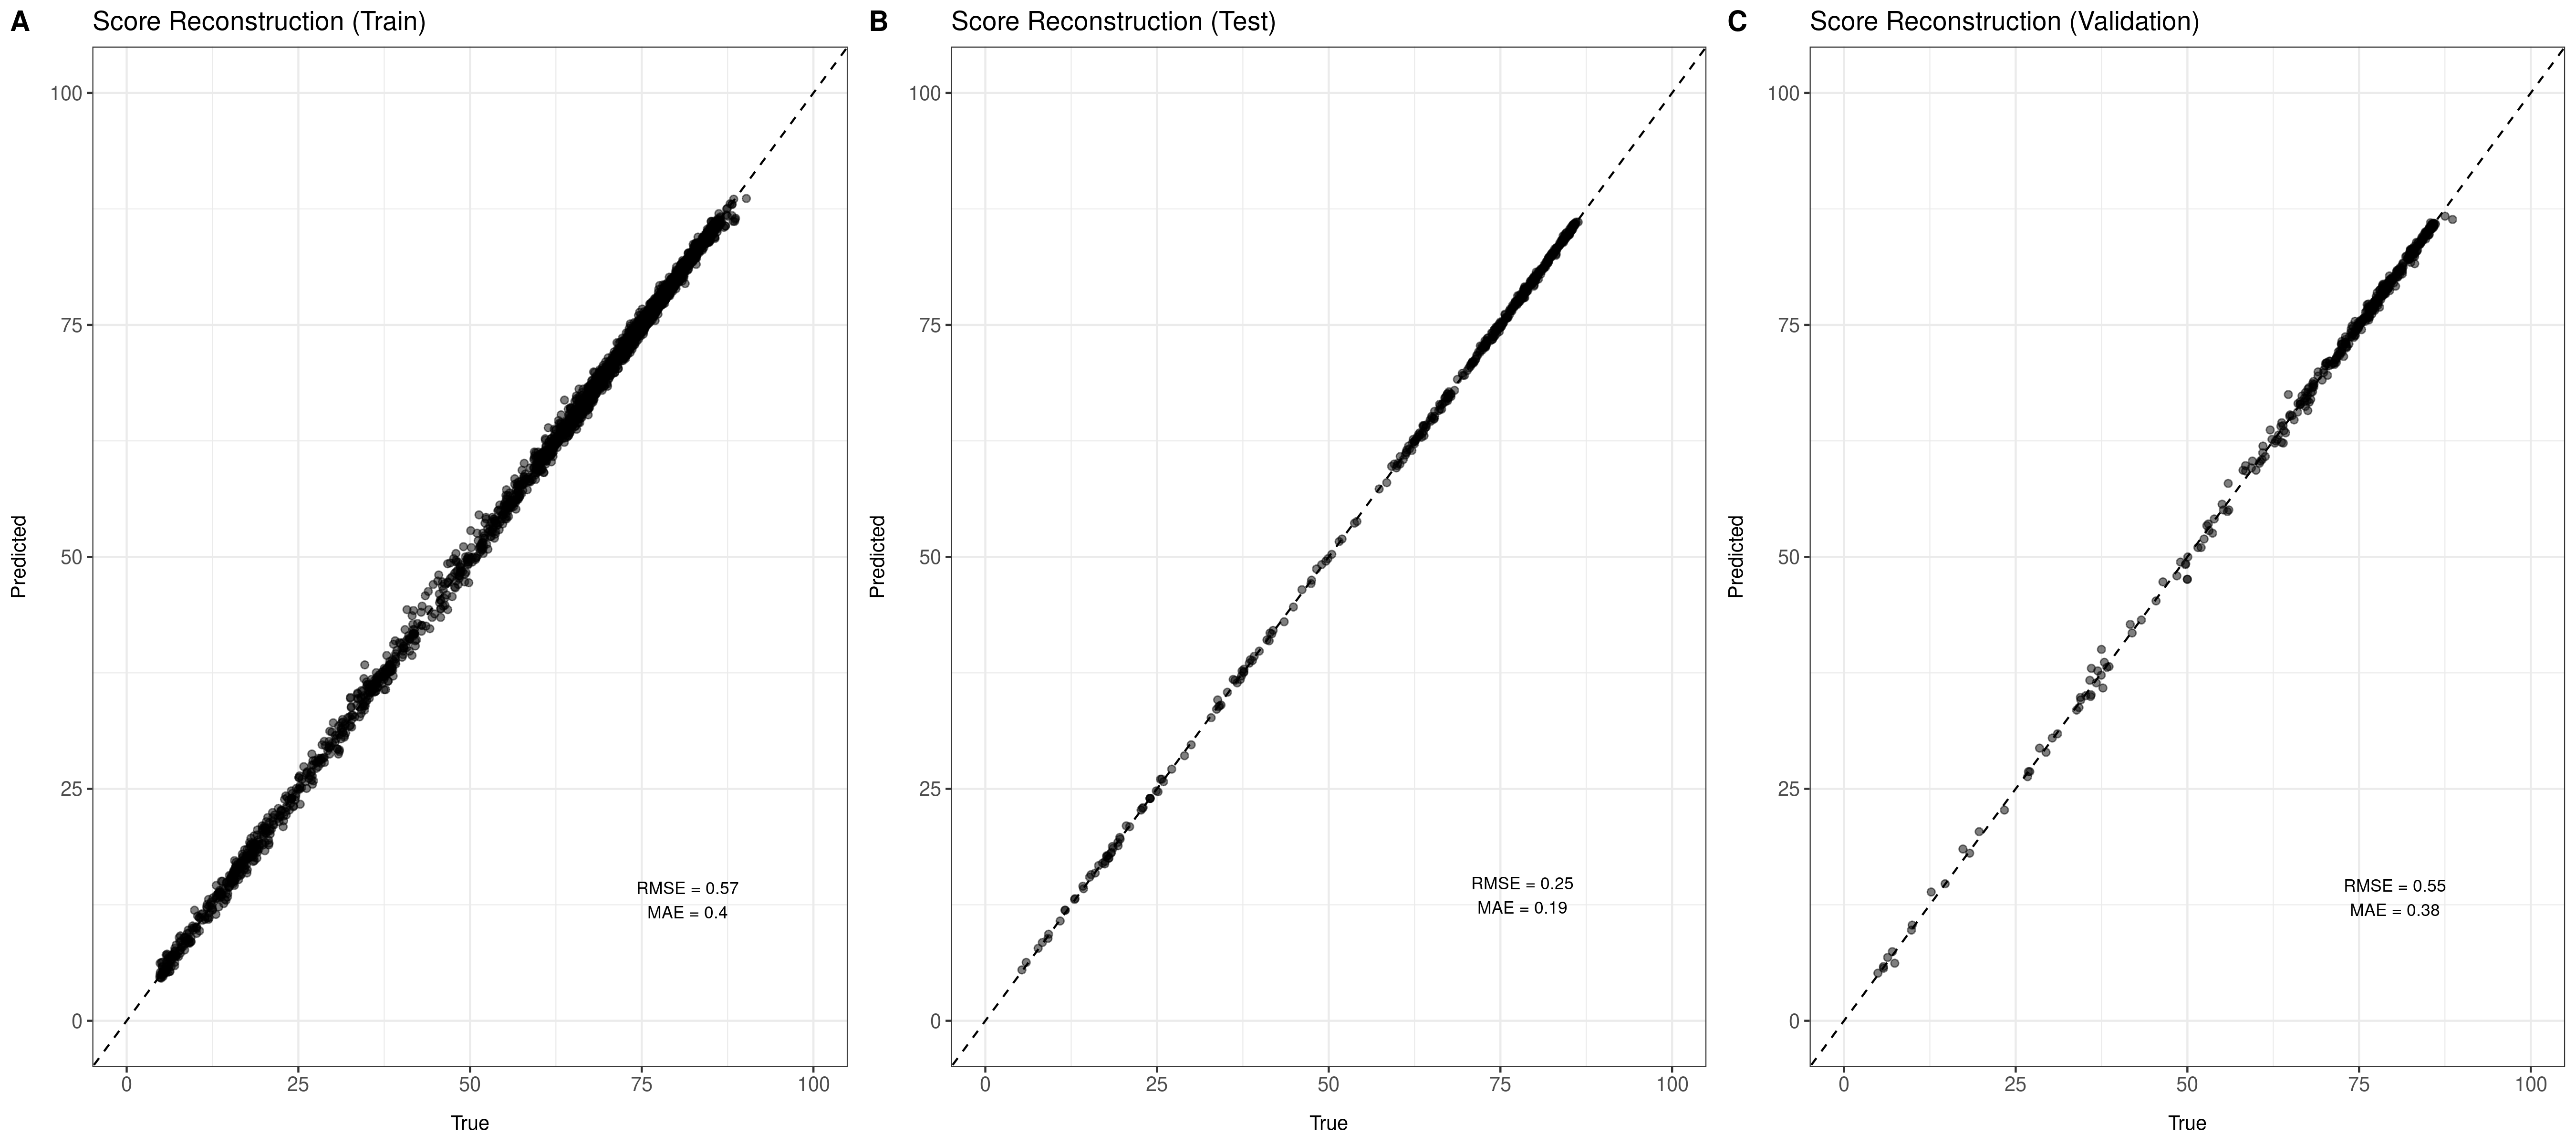
\includegraphics[width=0.8\textwidth]{figures/hellaswag-reduced.png}
   \caption{}
   \label{fig:hs-reduced}
\end{figure}

% begin algorithm
% \begin{algorithm}
% \caption{Evolutionary subsampling}\label{alg:evo}
% \KwIn{Response matrices from training resp. test set $\mathbf A \in \{0,1\}^{n \times d}$, original score vector for training resp. test set $\mathbf s_0$ resp. $\mathbf s_1$, maximum number of items $d^*$, step size $k$}
% \KwResult{Subsampled response matrix $\mathbf A^* \in \{0,1\}^{n \times d^*}$}
% \While{$ncol(\mathbf A) > d^*$}{
%    \For{$i \in 1, \ldots, 50$}{
%       $\mathbf A^* \leftarrow \texttt{randomlyDropColumns}(\mathbf A, k)$\;
%       $\hat{\mathbf s} \gets \texttt{meanOfRows}(\mathbf A^*);$
%
%    }
%    $\mathbf A \leftarrow \mathbf A^*$\;
% }
% \end{algorithm}
% x times: randomly throw out items and see how well we can reconstruct the original scores on a test set
% choose the best set of disposable items
% repeat until d >= 1/4 of the original size
% test on validation set
\subsection{Item Response Theory}
% basic idea
% 2PL, 3PL, 3PLu, 4PL
% fitting with full-information (EM with semiparametric density estimation)
% estimate theta posterior per model
% fit gam to recover full score
% test on validation set
\subsection{Information Filtering}
% item characteristic curves
% item information
% information sweep and bayesian hyperparameter optimization

% ------------------------------------------------------------------------------------
%  Results
\section{Score Reconstruction}
% reconstruction of individual scores
% reconstruction of total score
% exploratory factor analysis

% ------------------------------------------------------------------------------------
%  Discussion / Conclusion
\section{Going Beyond Point Scores}
\section{Conclusion}
\subsection{Limitations}
\subsection{Future Work}

% ------------------------------------------------------------------------------------
%  Appendix
\section*{Acknowledgments}
\section*{References}
\section*{Appendix}
\end{document}
